\section{System Architecture and Design}

\subsection{Overall Architecture}

The system follows a microservices architecture with the following main components:

\begin{figure}[h]
\centering
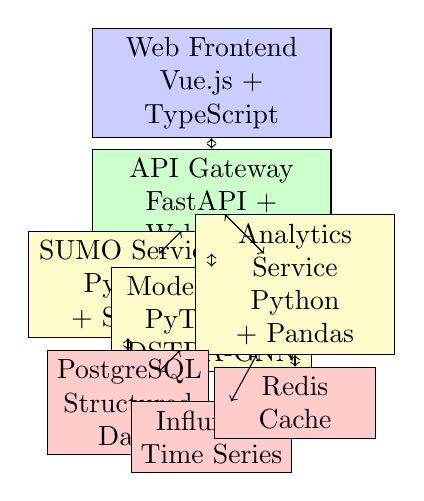
\begin{tikzpicture}[node distance=1.5cm, auto]
    % Frontend Layer
    \node[draw, rectangle, fill=blue!20, minimum width=3cm, text width=2.8cm, align=center] (frontend) {Web Frontend\\Vue.js + TypeScript};
    
    % API Gateway
    \node[draw, rectangle, fill=green!20, below of=frontend, minimum width=3cm, text width=2.8cm, align=center] (gateway) {API Gateway\\FastAPI + WebSocket};
    
    % Core Services
    \node[draw, rectangle, fill=yellow!20, below left of=gateway, minimum width=2.5cm, text width=2.3cm, align=center] (sim) {SUMO Service\\Python + SUMO};
    \node[draw, rectangle, fill=yellow!20, below of=gateway, minimum width=2.5cm, text width=2.3cm, align=center] (model) {Model Service\\PyTorch + DSTRA-GNN};
    \node[draw, rectangle, fill=yellow!20, below right of=gateway, minimum width=2.5cm, text width=2.3cm, align=center] (analytics) {Analytics Service\\Python + Pandas};
    
    % Data Layer
    \node[draw, rectangle, fill=red!20, below of=sim, minimum width=2cm, text width=1.8cm, align=center] (postgres) {PostgreSQL\\Structured Data};
    \node[draw, rectangle, fill=red!20, below of=model, minimum width=2cm, text width=1.8cm, align=center] (influx) {InfluxDB\\Time Series};
    \node[draw, rectangle, fill=red!20, below of=analytics, minimum width=2cm, text width=1.8cm, align=center] (redis) {Redis\\Cache};
    
    % Connections
    \draw[<->] (frontend) -- (gateway);
    \draw[<->] (gateway) -- (sim);
    \draw[<->] (gateway) -- (model);
    \draw[<->] (gateway) -- (analytics);
    \draw[<->] (sim) -- (postgres);
    \draw[<->] (model) -- (postgres);
    \draw[<->] (analytics) -- (influx);
    \draw[<->] (analytics) -- (redis);
\end{tikzpicture}
\caption{System Architecture Overview}
\label{fig:architecture}
\end{figure}

\subsection{Component Specifications}

\subsubsection{Web Frontend}

The frontend is built using modern web technologies:
\begin{itemize}
    \item \textbf{Framework}: Vue.js 18+ with TypeScript for type safety and component-based architecture
    \item \textbf{Key Features}:
    \begin{itemize}
        \item Interactive route selection on map
        \item Real-time traffic visualization
        \item ETA prediction display
        \item Statistical analysis dashboard
    \end{itemize}
    \item \textbf{Integration}: Mapbox GL JS for maps, Plotly.js for data visualization
    \item \textbf{Communication}: WebSocket for real-time updates from backend
\end{itemize}

\subsubsection{API Gateway}

The API Gateway serves as the central communication hub:
\begin{itemize}
    \item \textbf{Technology}: FastAPI framework with WebSocket support
    \item \textbf{Functions}:
    \begin{itemize}
        \item Request routing to appropriate microservices
        \item Authentication and authorization
        \item Rate limiting and throttling
        \item WebSocket connection management for real-time updates
    \end{itemize}
    \item \textbf{Protocols}: HTTP/REST for standard requests, WebSocket for streaming
\end{itemize}

\subsubsection{SUMO Service}

The SUMO service handles traffic simulation:
\begin{itemize}
    \item \textbf{Technology}: Python with SUMO-Simulation library
    \item \textbf{Functionality}:
    \begin{itemize}
        \item Initialize and control SUMO simulations
        \item Extract vehicle positions and states
        \item Monitor junction states and traffic lights
        \item Generate dynamic graph structures
    \end{itemize}
    \item \textbf{Interface}: TraCI (Traffic Control Interface) for real-time control
\end{itemize}

\subsubsection{Model Service}

The model service provides inference capabilities:
\begin{itemize}
    \item \textbf{Technology}: PyTorch-based inference engine
    \item \textbf{Functionality}:
    \begin{itemize}
        \item Load DSTRA-GNN model checkpoints
        \item Transform simulation data to graph format
        \item Perform real-time ETA predictions
        \item Cache predictions for performance
    \end{itemize}
    \item \textbf{Optimization}: Model quantization, batch processing, GPU acceleration
\end{itemize}

\subsection{Data Management Architecture}

\subsubsection{PostgreSQL Database}

Used for structured data storage:
\begin{itemize}
    \item Simulation configurations and metadata
    \item User sessions and routes
    \item Prediction results and ground truth
    \item Model metadata and versions
\end{itemize}

\subsubsection{InfluxDB Database}

Used for time-series data:
\begin{itemize}
    \item Vehicle positions and states over time
    \item Junction traffic volumes
    \item Real-time traffic metrics
    \item System performance metrics
\end{itemize}

\subsubsection{Redis Cache}

Used for high-speed data access:
\begin{itemize}
    \item Recently computed predictions
    \item Session state management
    \item Rate limiting counters
    \item WebSocket connection metadata
\end{itemize}

